Lets check whether $\div{\va{A}}$:
\begin{align*}
\grad_r \vdot {\int \frac{\va{j} (\va{r'}) \dd[3]{r'}}{\qty|\va{r} -\va{r'}|}} =  \int \grad_r \vdot \qty(\frac{\va{j} (\va{r'}) \dd[3]{r'}}{\qty|\va{r} -\va{r'}|})  = \int \dd[3]{r'}  \va{j} (\va{r'}) \grad_{r} \vdot \frac{1 }{\qty|\va{r} -\va{r'}|} = -\int \dd[3]{r'}  \va{j} (\va{r'}) \grad_{r'} \vdot \frac{1 }{\qty|\va{r} -\va{r'}|} =\\= -\int \dd[3]{r'}  \grad_{r'} \vdot \frac{\va{j} (\va{r'})  }{\qty|\va{r} -\va{r'}|} - \frac{1 }{\qty|\va{r} -\va{r'}|} \underbrace{\grad_{r'} \vdot \va{j} (\va{r'}) }_{0} = - \oint \frac{\va{j} (\va{r'})  }{\qty|\va{r} -\va{r'}|} \vdot \dd{\va{s}} = 0
\end{align*}
\paragraph{Stokes' theorem}
For some vector field $\va{V}$ and closed curve $\Gamma$:
$$\int \qty(\curl{\va{V}}) \vdot \dd{\va{s}} = \oint \va{V} \vdot \dd{\va{l}}$$

In our case we get
$$\int\limits_{S} \qty(\curl{\va{B}}) \vdot \dd{\va{s}} = \oint \va{B} \vdot \dd{\va{l}}$$
$$\frac{4\pi}{c}\int\limits_{S} \va{j} \vdot \dd{\va{s}} = \oint \va{B} \vdot \dd{\va{l}}$$
We denote $I = \int\limits_{S} \va{j} \vdot \dd{\va{s}}$, which is current.
$$\frac{4\pi}{c}I = \oint \va{B} \vdot \dd{\va{l}}$$
\subsection{Gauge transformation}
Suppose we have $\va{A}' = \va{A} + \grad{\psi}$. We get $\va{B} = \curl{\va{A}} = \curl{\va{A'}}$.
Suppose $\div{\va{A}} = \chi$. Then
$$\div{\va{A'}} = \div{\va{A}} + \laplacian{\psi}$$
If we want $\div{\va{A'}} = 0$, we get $\chi + \laplacian{\psi} = 0$. Thus we can find $\psi$ such that $\laplacian{\psi} = -\chi$ and we get $\div{\va{A'}} = 0$.

\paragraph{}
If 
$$\va{A} = \frac{1}{c} \int \dd[3]{r'} \frac{\va{j}(\va{r})}{\abs{\va{r}-\va{r'}}}$$
we can get
$$\va{B} = \curl{\va{A}} = \frac{1}{c} \int \dd[3]{r'} \va{j}(\va{r}') \cross \frac{\qty(\va{r}-\va{r'})}{\abs{\va{r}-\va{r'}}^3}$$
\subsection{Biot–Savart law}
Suppose we have current $I$ on some curve $l'$. Then magnetic field due to this current in point $\va{r}$ is
$$\dd{\va{B}(\va{r})} = \frac{I}{c} \dd{\va{l'}} \cross \frac{\va{r}-\va{r'}}{\abs{\va{r}-\va{r'}}^3}$$
\paragraph{Example}
Suppose we have infinite wire with current $I\vu{z}$. Then the magnetic fiend due to the wire is
$$\dd{\va{B}} = \frac{I}{c}\frac{\dd{z}\vu{z} \cross \qty(\va{r}-\va{r'})}{\abs{\va{r}-\va{r'}}^3} = \frac{I}{c} \frac{\dd{z} R \vu{y}}{[R^2+z^2]^{\frac{3}{2}}}$$
Thus
$$B = \frac{I}{c} \int_{-\infty}^{\infty} \frac{\dd{z}R}{[R^2+z^2]^{\frac{3}{2}}} = \frac{2I}{cR}$$

Alternatively
$$\frac{4\pi}{c}I = \oint \va{B}\cdot \dd{\va{l}} = B \cdot 2\pi R$$
$$B = \frac{2I}{cR}$$
\paragraph{Meissner effect} Superconducting material actively excludes magnetic fields from its interior. Thus $\curl{\va{B}} = 0$ and there are currents only on the edge.
\paragraph{Example}
Suppose we have a boundary between two materials, with fields $\va{B}_1$, $\va{B}_2$. 
\begin{center}
	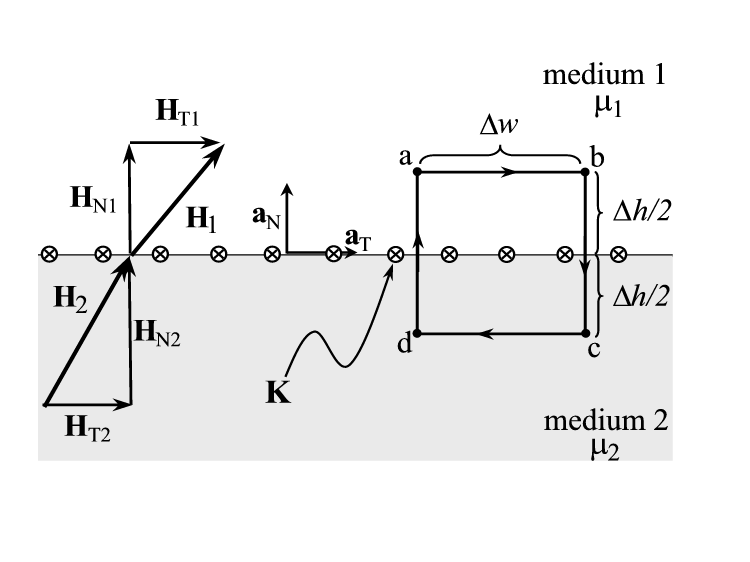
\includegraphics[width=0.5\linewidth]{./lect7/pic1.png}
\end{center}
Taking integral on small box on boudary we get
$$0 = \oint \div{\va{B}} \dd[3]{r} = \oint \va{B} \vdot \dd{s} = \qty(\va{B}_{1,\perp}-\va{B}_{2,\perp}) \Delta s$$
i.e. 
$$\va{B}_{1,\perp}=\va{B}_{2,\perp}$$

What happens with $B_\parallel$?

$$\oint \va{B}\vdot \dd{\va{l}} = \frac{4\pi}{c} \int \va{j} \vdot \dd{\va{s}} = I  = \frac{4\pi}{c} K \dd{l}$$
$$\qty(B_{2, \parallel} - B_{1, \parallel}) = \frac{4\pi}{c} \va{K}  \dd{l}$$
$$\vu{n} \cross (\va{B}_2 - \va{B}_1) = \frac{4\pi}{c} \va{K} $$
where $\va{K}$ is surface current density.
\paragraph{Magnetic scalar potential}
It's impossible to write $\va{B} = -\grad{\phi_m}$. However, if there is some area in which there is no current, we can try to do so, since $\curl{\va{B}} = 0$.
Using Biot-Savart law
$$\va{B}(\va{r})= \frac{I}{c} \oint \dd{\va{r'}} \cross \frac{\va{r}-\va{r'}}{\abs{\va{r}-\va{r'}}^3} = \frac{I}{c} \underbrace{\oint \dd{r'} \cross \underbrace{\va{U}(\va{r})}_{\frac{\va{r}-\va{r'}}{\abs{\va{r}-\va{r'}}^3}}}_{\va{H}}$$
For some constant vector $\va{k}$:
$$\va{k}\vdot \va{H} = \va{k} \vdot \oint \dd{\va{r'}} \cross \va{U}(\va{r}) = \oint \dd{\va{r'}} \vdot \qty(\va{U} \cross \va{k}  ) = \int \dd{\va{s}} \cdot \curl(\va{U} \cross \va{k}) = \int \dd{\va{s}} \cdot \qty[ (\va{k} \vdot \grad)\va{U} - \va{k} (\div{\va{U}})]$$